\documentclass{my}
%\documentclass{article}
\input{logicmacros}
\usepackage{url}


\ifx\pdfoutput\undefined
% we are running LaTeX, not pdflatex
\usepackage{graphicx}
\else
% we are running pdflatex, so convert .eps files to .pdf
%\usepackage[pdftex]{graphicx}
%\usepackage{epstopdf}
\fi 

\copyrightyear{}
\pubyear{}

\def\P1{\pr{P-1}}

\def\C{\pr{C}}
\def\O{\pr{O}}

\def\dr{\Longrightarrow}

\def\ObjectPropertyAxiom{\pr{ObjectPropertyAxiom}}
\def\SubClassOf{\pr{SubClassOf}}

\def\partOfT{\pr{part\_of$^T$}}
\def\partOf{\pr{part\_of}}
\def\hasPart{\pr{has\_part}}
\def\isA{\pr{is\_a}}
\def\during{\pr{during}}
\def\invDuring{\pr{inverseOf(during)}}
\def\instanceOf{\pr{instance\_of}}
\def\historyOf{\pr{history\_of}}
\def\derivesFrom{\pr{derives\_from}}
\def\adjacentTo{\pr{adjacent\_to}}

\def\existsAt{\pr{exists\_at}}

\def\partOfAtSomeTimes{\pr{part-of-at-some-times}}
\def\partOfAtAllTimes{\pr{part-of-at-all-times}}
\def\hasPartAtSomeTimes{\pr{has-part-at-some-times}}
\def\hasPartAtAllTimes{\pr{has-part-at-all-times}}
\def\hasPartAtAllTimesForWhichPartExists{\pr{has-part-} \pr{at-all-times-}\ \pr{for-which-part-exists}}
\def\partOfAtAllTimesForWhichWholeExists{\pr{part-of-} \pr{at-all-times-}\ \pr{for-which-whole-exists}}

\def\atAllTimes{\pr{at-all-times}}
\def\atSomeTimes{\pr{at-some-times}}
\def\atAllTimesForWhichPartnerExists{\pr{at-all-times-for-which-partner-exists}}

\def\CellNucleus{\pr{cell nucleus}}
\def\Cell{\pr{cell}}

\def\OBOREL{\textbf{OBO-REL}}

\newcommand{\tbleqn}[1]{
\begin{math}
\begin{aligned}[1]
#1
\end{aligned}
\end{math}
}

\begin{document}
\firstpage{1}

\title{Shadowboxing: Mirroring the TBox in the ABox}

\author{Christopher J. Mungall\,$^{1}$\footnote{to whom correspondence should be addressed}}
\address{$^{1}$Genomics Division, Lawrence Berkeley National Laboratory, MS84R017, 1 Cyclotron Road, Berkeley, CA 94720 USA}

\history{}

\editor{}

\maketitle

\begin{abstract}

OWL2 has a strict separation between classes (TBox) and the domain of
discourse (ABox). This separation generally works well for the tasks
that OWL is designed for, but there are scenarios where it is
desirable to model certain entities simultaneuously as classes and
individuals. Motivations include the different logical properties of
the ABox as well as the desire to have a simpler RDF representation
that aligns with conventional graph-oriented views of ontologies. Many
existing attempts to put the ontology in the ABox are ad-hoc or even
accidental, and suffer from limitations.

In this document we describe a method for modeling an OWL TBox inside
an ABox that is \emph{valid} with respect to the original ontology,
preserves a restricted but useful set of entailments, and allows for
certain kinds of entailment not possible in a TBox. The RDF
representation of this ABox aligns well with conventional graph
representations. It also opens up possibilities for alternate ways of
approaching the modeling of some domains that may not be best served
by class-oriented models.

\end{abstract}

\section{Introduction}

\subsection{ABoxes and TBoxes}

With traditional Description Logics, objects can belong to either the
TBox (``terminology'' box, i.e. set of \emph{classes}), the ABox
(``assertion'' box, i.e. set of \emph{individuals}) or the RBox (the
set of \emph{properties})\footnote{other object types not relevant for
  this paper}. The ABox is also known as the \emph{domain of
  discourse}. These two sets do not share members; OWL2 introduces the
notion of \emph{punning}, whereby the same name (i.e. IRI) can refer
to either a class or individual, but this is just a syntactic
convenience for sharing annotations. Logically, the interpretation of
a punned name is in fact two names, and the ABox-TBox distinction is
thus maintained.

The modeler must decide how to partition their objects of interest
into the TBox and ABox. This is often trivial, with the TBox
containing classes such as \pr{dog}, \pr{person}, \pr{city} and the
ABox containing individuals such as \pr{Fido}, \pr{Fred} and
\pr{Oakland} (see Fig \ref{fig:intro}).

%----------------------------------------
\begin{figure}
\center
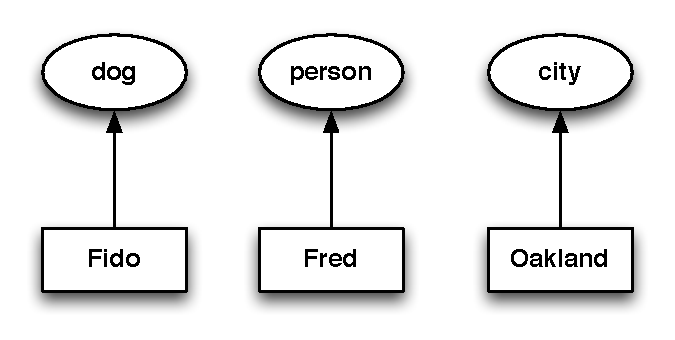
\includegraphics[width=7cm]{intro}
\caption{Separation of ABox (individuals, boxes) and TBox (classes,
  ovals) in a trivial ontology. }.
\label{fig:into}
\end{figure}
%----------------------------------------


The choice is not always straightforward. In the biological domain,
persuasive arguments exist for whether genes or species should be
modeled in the ABox or TBox (or both), and the modeler may be guided
by a variety of considerations, including philosophical principles or
practical modeling consequences based on the differing logical
properties of the ABox and TBox and the kinds of reasoning tasks
supported.

Modeling in the ABox provides certain advantages - examples include:

\begin{enumerate}

\item Objects in the ABox are in the domain of discourse. They are
  more readily queryable.

\item The ABox supports cyclic structures. In contrast, without
  extensions such as DL graphs, the TBox has the constraint that
  models must be trees. This means it is impossible to provide a
  complete description that classifies cyclic molecules (e.g. benzene)
  in the TBox. (see Dumontier 2007\cite{Dumontier2007})

\item Mapping an ABox to RDF does not introduce new blank nodes - in
  contrast, mapping a TBox to RDF frequently introduces new blank
  nodes, introducing a ``striping'' pattern in the corresponding RDF
  graph (see next section).

\end{enumerate}

Of course, if we over-model in the ABox we lose the ability to
classify individuals, to entail subclass relationships and to detect
unsatisfiability of classes - tasks that are vital in modern ontology
construction and use and one of the main motivations for using OWL in
the first place.

\subsection{OWL, RDF and Graphs}

Ontologies are commonly conceived of in graph-theoretic terms; for
example, the seminal Gene Ontology paper\cite{Ashburner2000} uses the
datamodel of a Directed Acyclic Graph, and most bioinformatic tools
and relational databases use a graph model to represent the
ontology\cite{Mungall2007}. We define a \emph{simple graph mapping} (SGM) of
an ontology $O$ to a graph $G = <V,E>$ as one in which each class is
mapped to a vertex $V$ in the graph, with axioms connecting two
classes being mapped to an edge $E$. A property of the SGM is that no
new nodes are introduced.

RDF (Resource Description Framework) is a subset of first-order logic
consisting of ``subject-predicate-object triples'' i.e. predicate
sentences with two arguments. This has a natural mapping to a graph
$G$, with each triple $<S P O>$ forming an edge $E$ between source
node $S$ and target node $O$ labeled by $P$.

An OWL ontology can be represented as an RDF graph, i.e. a set of
triples. There is a standard serialization into triples provided by
the W3 recommendation \emph{mapping to
  rdf}\footnote{http://www.w3.org/TR/owl2-mapping-to-rdf/}. The
mapping of OWL to RDF to a graph is not an SGM, as the following
example shows.

Under the W3C mapping, a single existential axiom of the
form\footnote{We use Manchester Syntax to write OWL axioms}:

\begin{verbatim}
X SubClassOf R some Y
\end{verbatim}

Is mapped to 4 triples\footnote{We use n-triples format to write RDF}

\begin{verbatim}
X rdfs:subClassOf _:1 .
_:1 a owl:Restriction .
_:1 owl:onProperty R .
_:1 owl:someValuesFrom Y /
\end{verbatim}

This can become verbose where ontologies contain multiple such
existential axioms (as is standard for most bio-ontologies -
e.g. partonomies in anatomical ontologies). This can be a hindrance
when working with ontologies using RDF tools that do not support an
OWL syntactic sugar layer, or in using technologies designed for
reasoning over triples. See figure \ref{fig:partonomy} for an illustration.

%----------------------------------------
\begin{figure}
\center
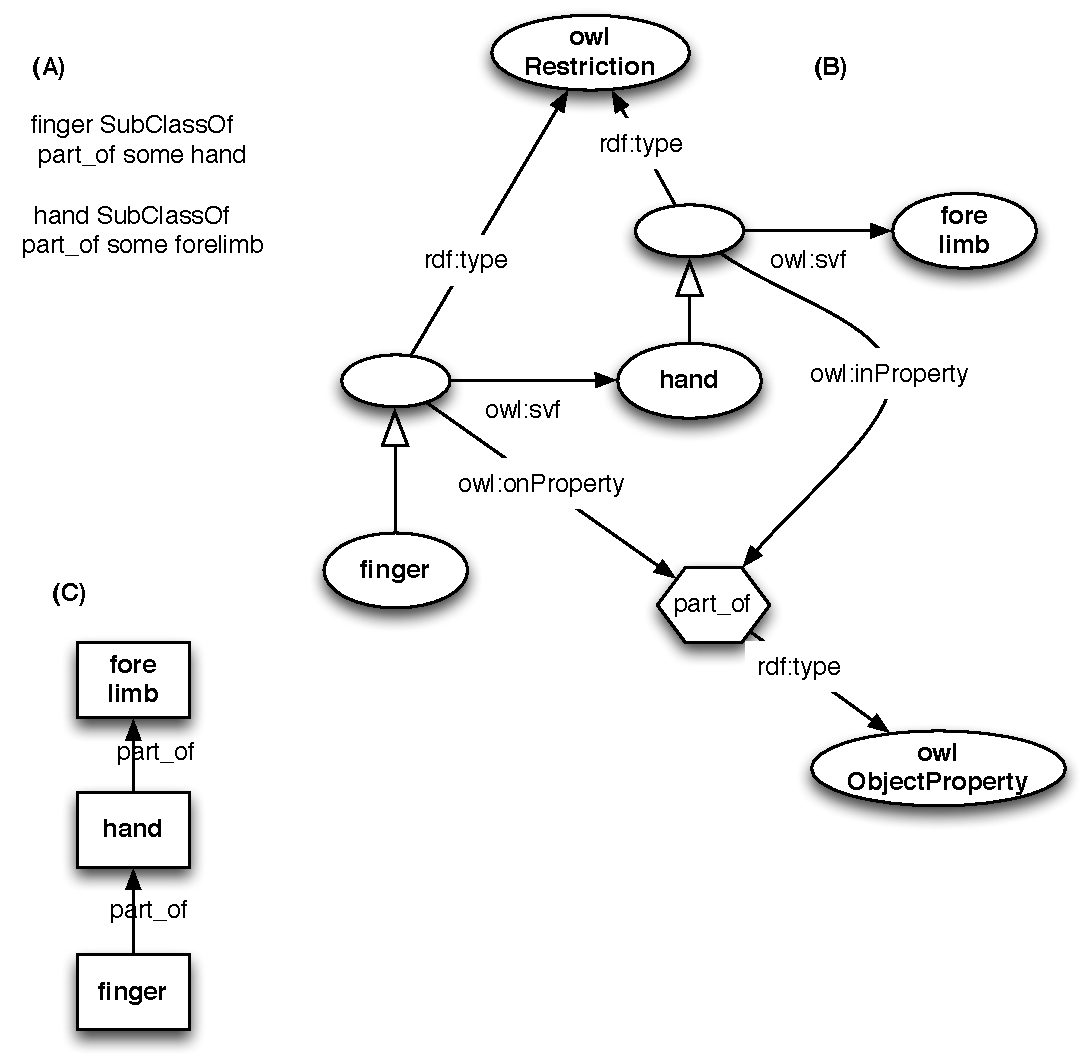
\includegraphics[width=7cm]{partonomy}
\caption{Example two-class partonomy represented in (A) OWL Manchester
  Syntax and (B) the semantically identical RDF-level
  representation. (C) shows a naive translation to a simple graph, in
  which the classes are mapped to the ABox, and class axioms become
  object property assertions.}
\label{fig:partonomy}
\end{figure}
%----------------------------------------


It is also problematic when the RDF representation of the OWL is
directly mapped to a graph when using graph-based software
(e.g. visualization tools such as cytoscape or graph databases such as
Neo-4j). This is because the ``striping'' above essentially produces a
bipartite graph, rather than a ``clean'' graph as outlined above.

%In biological ontologies, these existential axioms are common, and are
%commonly conceived of as a single edge in a graph whose nodes are
%classes, with each edge X-Y labeled with R.

\subsection{Naive ABoxification leads to incoherency}

Many knowledge bases (e.g. Freebase; Neurolex) use a simple form of
knowledge representation where concepts are linked via triples,
eschewing more formally specified OWL axioms and attendant reasoning
benefits.

We may be tempted to map an OWL ontology to triples in a more direct
fashion:

\begin{verbatim}
X SubClassOf R some Y <==> <X R Y> .
\end{verbatim}

The problem with this naive translation is that it leads to
\emph{incoherent} ontologies - i.e. ontologies that contain
unsatisfiable classes. E.g. consider the following biologically
accurate and coherent 4-axiom ontology:

\begin{verbatim}
Class: nucleus
 SubClassOf: hasPart some chromosome
Class: mitochondrion 
 SubClassOf: hasPart some chromosome
ObjectProperty: hasPart
  InverseOf: partOf
Axiom:
(partOf some nucleus) 
  DisjointWith 
(partOf some mitochondrion)
\end{verbatim}

The first two axioms\footnote{we leave as open for now the question of
  how to map axioms such as Disjointness axioms} are translated as

\begin{verbatim}
<nucleus hasPart chromosome> .
<mitochondrion hasPart chromosome> .
\end{verbatim}

Because of the inverse properties axiom we entail

\begin{verbatim}
<chromosome partOf nucleus> .
<chromosome partOf mitochondrion> .
\end{verbatim}

If we translate these back to OWL using the naive translation, we end
up with an incoherent ontology (because \emph{nucleus} and
\emph{chromosome} are entailed to be equivalent to Nothing):

\begin{verbatim}
Class: chromosome
 SubClassOf: partOf some nucleus
 SubClassOf: partOf some mitochondrion
ObjectProperty: hasPart
  InverseOf: partOf
Axiom:
(partOf some nucleus) 
  DisjointWith 
(partOf some mitochondrion)
\end{verbatim}

Even when translating in one direction, we can end up with undesired
inferences (e.g. consider domain and range constraints).

Despite this problem, the naive translation is sometimes used where
there is a desire to have a simpler RDF reqpresentation.

\subsection{Requirements for a graph mapping of OWL2}

Our requirements for a mapping from OWL2 to a graph are:

\begin{enumerate}

\item aligns with a basic graph representation (does not introduce
  blank nodes and striping)

\item coherency-preserving

\item preserves entailments where possible

\item supplements standard W3C translation rather than replaces it

\end{enumerate}

The standard W3C mapping to RDF preserves coherency and many
entailments - but violates the first requirement by introducing blank
nodes for existential restrictions.

The naive translation succeeds with the first requirement, but fails
to preserve coherency (and consequently fails to preserve
entailments?). 

\section{TBox shadowing}

We introduce a method callsed TBox shadowing. This is very similar to
the naive translation, but introduces a mapping at the level of object
properties to preserve coherency.

\subsection{Preliminaries}

\subsubsection{Graphs}

\subsubsection{RDF}

\subsubsection{OWL-DL}

\subsubsection{OWL-Full}

\subsection{Translation of Class Axioms}

Each class $C$ in $O$ is mapped a named individual $C$ in $O'$. The
same name (IRI) is used - this means that if O and O' are combined we
have /emph{punning}.

A subset of class axioms in $O$ are translated to \ObjectPropertyAxiom
s in $O'$

\begin{verbatim}
A SubClassOf B ==> OPE(A SubClassOf' B)
A SubClassOf R some B ==> OPE(A R' B)
\end{verbatim}

Strictly speaking the $A$ and the $B$ classes on the LHS are different
objects from the $A$ and $B$ individuals on the RHS, but we use OWL2
punning in our notation here.

Here $R'$ denotes a type-level counterpart or shadow of $R$. Note that
punning is \emph{not} used here $R'$ is a truly distinct name (IRI)
from $R$. Both $R$ and $R'$ are ObjectProperties.

\SubClassOf' is an
OWL2-DL ObjectProperty that is a type-level counterpart of the
RDFS/OWL-Full \pr{rdfs:subClassOf} property

We introduce two property chain axioms for every shadowed property
$R'$:

\begin{verbatim}
R' o SubClassOf' ==> R'
SubClassOf' o R' ==> R'
\end{verbatim}

Together with:

\begin{verbatim}
Transitive(SubClassOf')
Reflexive(SubClassOf')
AntiSymmetric(SubClassOf')
\end{verbatim}

To illustrate, consider an ontology $O'$ is:

\begin{verbatim}
A SubClassOf B
B SubClassOf partOf some C
C SubClassOf D
\end{verbatim}

Then $O'$ entails 

\begin{verbatim}
<A partOf' D>
\end{verbatim}

\subsubsection{Conherency Proof} TODO: Proof that this is
coherency-preserving. Intuitively this is the case as subclass
inferences propagate over existentials.

\subsection{Translation of Object Property Axioms}

A subset of axioms for R are also shadowed:

\begin{verbatim}
Transitive(R) ==> Transitive(R')
R <- R1 o ... o Rn ==> R'<- R1' o ... o Rn'
\end{verbatim}

\subsubsection{Conherency Proof} TODO: Proof that this is coherency-preserbing

\subsubsection{Propagation of symmetry axioms introduces incoherency}
TODO: Example. E.g. nucleus adjacentTo cytoplasm.

\subsubsection{Propagation of inverse axioms introduces incoherency}
See example in introduction

\subsection{Translation of equivalence axioms}

Equivalence axioms currently have an incomplete translation. Currently only "genus-differentia" style
are translated:



\begin{verbatim}
X = G and R1 some Y1 and ..
==>
X sameAs GenId
GenId SubClassOf' G
GenId R1' Y1,
....
\end{verbatim}

Where GenId is an auto-generated IRI (e.g. using a UUID) to avoid falling outside OWL2

TODO: this relies on CWA, need to explicitly close the world

\subsection{Translation of annotation axioms}

Because the same names (IRIs) are used for classes, each class $C$ in
$O'$ should have the same annotations, if $O'$ extends $O$.

However, care must be taken in copying annotations from an object
property $R$ to its shadow $R'$.

Annotations are logically silent, so propagation will not affect
entailment. However, annotations should not be propagated blindly as
this could cause confusion. We recommend some kind of syntactic
pattern for translation of object proeprty annotations involving
certain annotation properties such as rdfs:label.

\section{Implementation}

A preliminary implementation is available in
OWLTools\footnote{http://owltools.googlecode.com}.

The class name is
owltools.mooncat.OWLInAboxTranslator\footnote{http://owltools.googlecode.com/ 
svn/trunk/docs/api/owltools/mooncat/ OWLInAboxTranslator.html}

To run:
\begin{verbatim}
owltools my.owl --tbox-to-abox -o my-abox.owl
\end{verbatim}

The translation by default generates label annotations for shadowed
object properties, suffixing them with ``type level''.

The method \pr{trTypeLevel} will generate a name $R'$ shadowing an
object property $R$. Currently it does this by suffixing the IRI with
the string ``TLR'', but in future this may be configurable.

The \SubClassOf' object property is the same translation applied to
the IRI for rdfs:subClassOf (this may be changed in the future).

\section{OWL2 Profile of shadowed TBox}

The shadowed TBox falls in the EL++ subset, which allows use of fast
reasoners such as Elk.

In addition, the the kinds of simple entailment supported by many
triplestores becomes more useful with a shadowed TBox in comparison to
the W3C translation.

Note that shadowing loses axioms. For many applications this may not
matter. For example, an ontology $O$ can be validated and
pre-classified using OWL reasoners, with direct inferred axioms added
to make $O_2$, and then applications consume $O_2'$.

\section{Applications}

\subsection{SPARQL queries}

The standard W3C mapping of OWL to RDF results in additional blank
nodes and striping, making basic SPARQL queries difficult. In
addition, the simple entailment regimes provided with some SPARQL
engines may be incapable of basic inferences, such as those combining
transitivity of object properties and existential axioms. These are at
the core of many biological ontologies, which often have a partonomy
as the backbone (e.g. neuro-anatomy), or somelines an ontogenic
lineage (e.g. cell ontologies).

For these reasons, many triplestores eschew an OWL2 TBox
representation, and use triples to connect the representational
units. This is typically done in an ad-hoc way without thought to the
OWL2 semantics, sometimes resulting in accidentally falling into
OWL-Full, sometimes limiting the use of the knowledge base for complex
queries etc. Examples include dbpedia, freebase, the neurolex
triplestore. The Non-DL OWL translation of the FMA can be considered
to fall into this category.

TODO - compare queries.

TODO - example query from Neurolex paper

\subsection{Finding ancestors}

It is surprisingly difficult to query a conventional TBox ontology for
descendants over any relationship type. In OWL2 this is can be
specified as finding $y$ and $r$ where

\begin{verbatim}
?x SubClassOf ?r some ?y
\end{verbatim}

For a given $x$. In practical terms this query must typically be
answered by first seeding the ontology with classes for the form ``?r
some ?y'' and then performing a superclass query.

In contrast, if the existential axioms are shadowed as triples, this
becomes a query for a single assertion:

\begin{verbatim}
?x ?r' ?y
\end{verbatim}

Which can be performed easily with the OWLAPI. In addition, the
corresponding SPARQL query is simple, and the required entailment only
requires a limited number of property chains in most cases.

\subsection{Mapping to graph databases}

TBox shadowing provides one way to map an OWL ontology to graph
databases such as Neo4j, and to graph-based visualization tools such
as Cytoscape.

Whilst it would be possible to simply use the naive translation (Neo4j
models do not have a formal set-theoretic or first order logic
interpretation, so there is no danger of introducing incoherency),
using the TBox shadowing mapping has the advantage of having a
simultaneous direct RDF translation of the Neo4j that is coherent. The
cost is the introduction of an object property mapping.

Non-RDF graph models often allow multiple labels, so another
alternative is to annotate the edge with logical properties. For
example, an existential restriction axiom may be mapped to a single
edge annotated with both the object property and the expression type
(ObjectSomeValuesFrom). 

\subsection{Formalization of Type-Level Relations}

[out of scope for this paper?]

The OBO Relations Ontology paper from 2005\cite{Smith2005} formalized
a set of binary type level relations in terms of instance-level binary
or ternary (time-indexed) relations. In this formalization,
classification units such as ``cell'' and ``cell nucleus'' are
conceived of as ``types'' or ``universals'', and are considered to be
part of the domain of discourse.

For example, the logic sentence ``CellNucleus \emph{part of} Cell''
(using the 2-argument type-level part-of relation) has an interpretation:

$
\A x \A t : \instanceOf(x, \CellNucleus, t) \imp \\
 \E y \instanceOf(y, \Cell, t), \partOf(x,y,t)
$

There is no agreed-upon alignment of the RO 2005 paper with
OWL. Whilst the type-level relationships (such as that between nucleus
and cell) might naturally by represented using a single triple, this
was generally eschewed by ontologies using OWL, and instead
existential restrictions were used\cite{golbreich2007obo}, in order to
maximize use of OWL and OWL reasoners. However, this approach has
problems as it introduces binary instance-level relations whose
temporal interpretation is not clear.

The TBox shadowing strategy outlined in this document could be used to
provide a partial alignment of RO-2005 to OWL.

Here, the RO-2005 notion of ``type level relation'' corresponds
directly to shadowed object properties, and the punned class names
correspond to universals/types (which are in the domain of
discourse).

Under this interpretation, the shadowed TBox axioms in the ontology
$O'$ would be conceived of as the primary or canonical OWL
representation of the ontology. The corresponding TBox representation
would be conceived of as a derived artifact that can be used in
conjunction with OWL tools and OWL reasoners.

This is just a preliminary sketch of the approach - it does not
address time-indexed instance level relations, and it leaves open the
possibility of different kinds of temporal quantification for the type
level relations (e.g. there may be a TLR for at-some-times as well as
at-all-times).

\subsection{Phylogenetic trees}

\subsection{Anatomical structures and homology}

A standard OWL2 anatomical ontology uses classes to represent
generalizations of particular anatomical structures in the world. For
example, the class ``finger'' is instantiated by all actual fingers,
such as my left middle finger.

This is obviously useful for OWL reasoning, but placing the
generalized structures outside the domain of discourse has some
consequences when the generalized structures are themselves the
subject of study as opposed to groupings for data.

For example, evolutionary developmental biology is concerned with how
structures such as the limb or the digits have changed (or are
preserved) over deep time. In a conventional TBox representation, all
class axioms hold over the individual structures themselves - my left
forelimb, the pectoral fin of this particular fish instance - not
about the patterns observed at the level of individual
species. Homology is often conceived of in terms of these patterns
(Van Valen).

One practical consequence is in recording homology statements. With a
TBox representation, the axiom

\begin{verbatim}
forelimb SubClassOf 
  homologousTo some 'pectoral fin'
\end{verbatim}

does \emph{not} entail:

\begin{verbatim}
'pectoral fin' SubClassOf 
  homologousTo some forelimb
\end{verbatim}

This is somewhat unsatisfactory, as we are forced to make reciprocal
assertions (there are no situations where the reciprocal axiom would
not be true). This is not a major issue, something easily addressed
with a patina of additional tooling. But it does hint that we are
working at the wrong level of abstraction and we need the anatomical
structures to be in the domain of discourse. Then we could simply
write:

\begin{verbatim}
OPE(forelimb homologousTo' 'pectoral fin')
Symmetric(homologousTo')
\end{verbatim}

And get the correct entailments. 

The TBox shadowing provides a mechanism for doing this. Anatomy
ontologies can continue to be authored as conventional TBox
ontologies. Entailments from $O'$ can be reverse-shadowed back into
$O$ (giving a more formal mechanism for ensuring TBox homology axioms
are reciprocated). Or in fact $O'$ could be regarded as the canonical
representation. This has some philosophical appeal, if one conceives
of evolution as being about changes in patterns.

There may be additional expressivity gains beyond symmetricality of
assertions. MORE TO BE WRITTEN HERE

\subsection{Genes and proteins}

There are various tradeoffs when deciding whether to model specific
genes (such as ``human alpha-synuclein gene'') in the TBox or
ABox. Some are fairly prosaic yet important - e.g. if the TBox is
conceived of by some tools as the ``terminology box'' then a TBox
representation allows use of some terminology tools. Other reasons
pertains to the kinds of entailments desired and the kinds of
questions asked. Or an approach based in ontological realism may be
preferred, with distinctions drawn between physical molecule regions,
information content entities, and mind-independent generically
dependent continuants.

To see some of the practical considerations, consider a TBox model
(for example, the PRO ontology, which is class based, with the
individuals being actual protein molecule instances - one can easily
conceive of a gene parallel to this).

How do we answer the question ``how many genes does a human have''?
This question is strictly speaking underspecified - one could answer
with the number of distinct physical DNA portions with coding
potential in a given human, which would be in the trillions. But this
would be perverse. Typically we are interested in the interpretation
that yields an answer of the order 20-30k (ignoring for now
interesting but not relevant questions of biochemically active but
unselected DNA, etc).

It is difficult to get a TBox model to yield this answer. The reason
being we are implicitly interested in a particular level of
specificity - SHH, SNCA, PINK1, ... these are all ``distinct'' genes
at the right level of specificity. ``developmental gene'' or
``synuclein family gene'' are not - yet these are valid classes in the
TBox model.

THIS IS GETTING TOO WAFFLY...

ADD EXAMPLE INVOLVING PHYLOGENETIC TREES

\section{Discussion}

Even in an OWL environment, answering questions such as "what are the descendants of 'finger'" and
receiving a \partOf\ edge to 'limb' are not directly supported in OWL reasoners - it is necessary to
materialize R-some-Y classes.

More generally, because classes are part of the TBox and not in the domain of discourse, certain
kinds of queries are harder. These include queries for homologous structures, where these structures
are traditionally represented as classes.


\section{Conclusions}


%\section*{References}

% ========================================
\bibliography{tbox2abox}
\bibliographystyle{plain}
% ========================================

\newpage
\section*{Appendix}


\end{document}
